\chapter{Segnali periodici nel dominio della frequenza}

\begin{figure}[h]
    \centering
    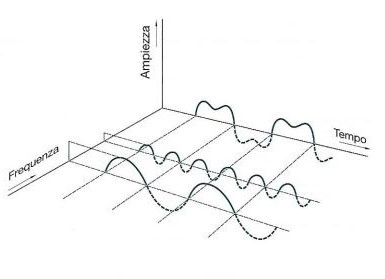
\includegraphics{Tempo frequenza segnale periodico tagliato.jpg}
\end{figure}  

\newpage 

\section{Sviluppo in serie di Fourier}

Diverse volte è utile osservare lo stesso segnale in altre rappresentazioni equivalenti. \newline 

Per rappresentazione di un segnale si intende una qualsiasi modalità idonea alla sua individuazine 
biunivoca. \newline 

La rappresentazione può comportare un cambiamento del dominio di definizione. \newline  

Quindi, grazie ad una rappresentazione, si può passare da un dominio all'altro dello stesso segnale. \newline 

Se il segnale s(t) è periodico con periodo T e pulsazione fondamentale $\omega_0$, possiamo definire una rappresentazione 
nota come Sviluppo in serie di Fourier. \newline 

Il dominio non sarà il tempo, bensì la frequenza (cioè l'inverso del tempo). \newline 

s(t) può essere visto come, grazie alla formula di sintesi dello sviluppo in serie di Fourier: \newline

{
    \Large 
    \begin{equation}
        s(t) 
        = 
        \sum_{k = - \infty}^{\infty} 
        C_k \frac{1}{\sqrt{T}} e^{\jmath \kappa \omega_0 t}
    \end{equation}
}

in cui: \newline

{
    \Large 
    \begin{equation}
        \omega_0 = \frac{2 \pi}{T}
    \end{equation}
}

e $C_k$ viene calcolato dall'analisi dello sviluppo in serie di Fourier: \newline

{
    \Large 
    \begin{equation}
        C_k 
        =
        \frac{1}{\sqrt{T}} \int_{-\frac{T}{2}}^{\frac{T}{2}} 
        s(t) e^{- \jmath \kappa \omega_0 t} dt
    \end{equation}
}

Ricordando, dalla matematica: 

{
    \Large 
    \begin{equation}
        \jmath ^{2} = -1 
    \end{equation}
}


 $e^{\jmath \kappa \omega_0 t}$ rappresenta una sinusoide e ponendo: 

{
    \Large 
    \begin{equation}
        \omega_k = k \omega_0
    \end{equation}
}

possiamo dire che qualsiasi segnale s(t) può essere visto come una 
successione di sinusoidi di diversa pulsazione. \newline 

In formule: 

{
    \Large 
    \begin{equation}
        s(t) \leftrightarrow \{C_k\}
    \end{equation}
}

dove per $\{C_k\}$ si intendene la lista dei coefficienti che formulano il segnale s(t). \newline 


Siccome $\{C_k\}$ sono dei coefficienti che rappresentano delle sinusoidi, 
i coefficienti avranno una parte reale e una parte immmaginaria. \newline 

Il singolo coefficiente $C_k$ avrà la parte reale, 
scritta come $\Re[C_k]$ oppure $\abs{C_k}$, e la parte immmaginaria del coeffieciente 
sarà indicata come $\Im[C_k]$ oppure $\arg[C_k]$. \newline 

$\abs{C_k}$ prende anche il nome di modulo di $C_k$, 
mentre $\arg[C_k]$ prende il nome di fase di $C_K$. \newline 

Dal punto di vista grafico, possiamo visualizzare tutti i moduli e le fasi dei coeffiecienti $C_k$ 
usando lo spettro. \newline 

Lo spettro dei moduli di $C_k$ prende il nome di spettro di ampiezza, 
mentre lo spettro delle fasi prende il nome di spettro di fase. \newline 

Un esempio di spettro di ampiezza e spettro di fase: 

\begin{figure}[h]
    \centering
    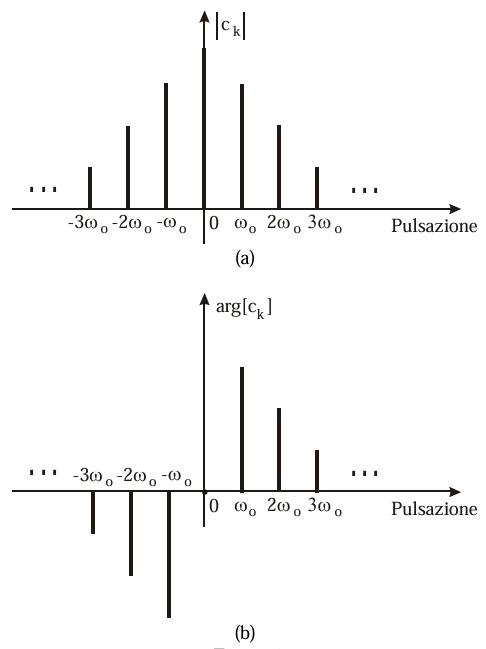
\includegraphics{Esempio di spettro di ampiezza e di fase.PNG}
\end{figure} 

Come si vede dalla figura, nello sviluppo in serie di Fourier, 
gli spettri sono a righe perchè le armoniche sono discrete, armoniche multiple della frequenza fondamentale. \newline 

Con i puntini si intendono armoniche infinite, nella realtà si prenderanno le armoniche significative.  

\newpage 

\section{Criterio di Dirichlet} 

Dal punto di vista matematico, non tutti i segnali periodici possono essere rappresentati 
usando la rappresentazione della serie di Fourier. \newline 

Il segnale s(t) deve soddisfare il criterio di Dirichlet cioè: 

\begin{itemize}
    \item se s(t) è assolutamente integrabile sul periodo T, o in formula: 
    \begin{equation}
        \int_{-\frac{T}{2}}^{\frac{T}{2}} \abs{s(t)} dt < \infty
    \end{equation}
    \item se s(t) è continua o presenta un numero finito di punti di discontinuità di prima specie 
    \item se s(t) presenta in un periodo T un numero finito di massimi e minimi 
\end{itemize}

allora, se s(t) soddisfa questi criteri, la serie di Fourier converge al valore assunto dalla funzione
s(t) nei punti in cui questa è continua e alla semisomma del limite destro e sinitro nei punti in cui s(t) presenta le 
eventuali discontinuità di prima specie. \newline 

I segnali che vedremo nel corso soddisferanno il criterio di Dirichlet. \newline  

\newpage    

\section{Ortogonalità tra due segnali} 

Due segnali $x_1 (t)$ e $x_2 (t)$, in genere complessi, risultano ortogonali 
nell'intervallo $A \le t \le B$ se: 

{
    \Large 
    \begin{equation}
        \int_{A}^{B} 
        x_1 (t) x_2 ^{*} (t) dt = 0 
    \end{equation}
}

in cui il simbolo $*$ indica l'operazione di coniugato complesso. \newline 

Un esempio di sequenze ortogonali: 

\begin{figure}[h]
    \centering
    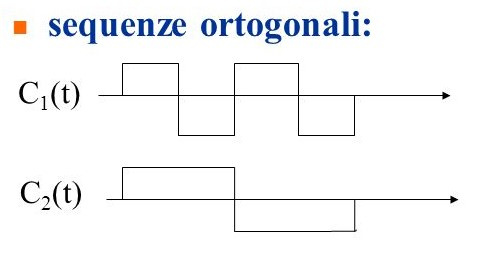
\includegraphics[scale = 0.8]{Segnali ortogonali.jpg}
\end{figure}  

Possiamo avere anche che: 

{
    \Large 
    \begin{equation}
        \begin{cases}
            A = -\infty \\
            B = \infty
        \end{cases} 
    \end{equation}
} 

Nel caso specifico, la condizione di ortogonalità tra due generiche funzioni espansione 
è verificata: 

{
    \Large 
    \begin{equation}
        \int_{-\frac{T}{2}}^{\frac{T}{2}} 
        e^{\jmath \kappa \omega_0 t} e^{-\jmath h \omega_0 t} 
        = 
        \begin{cases}
            T \text{    se  } h = k\\ 
            0 \text{    se  } h \neq k 
        \end{cases}
    \end{equation}
}

Questa equazione è valida solo se s(t) è un segnale reale. \newline 

\newpage

\section{Come ricavare moduli e fase in una serie di Fourier} 

Grazie alle formule di Eulero, possiamo scrivere la formula di sintesi della Serie di Fourier da: 

{
    \Large 
    \begin{equation}
        s(t) 
        = 
        \sum_{\kappa = - \infty}^{\infty} 
        C_k \frac{1}{\sqrt{T}} e^{\jmath \kappa \omega_0 t}
    \end{equation}
} 

Essendo un segnale s(t) reale, e che quindi per $\kappa \le 0$ si rispecchia quello che succede in $\kappa \ge 0$, 
la sommatoria possiamo scriverla da $\kappa \ge 0$, cioè: 

{
    \Large 
    \begin{equation}
        s(t) = \frac{a_0}{2} 
        +
        \sum_{\kappa = 1}^{+ \infty} [a_\kappa \cos(\kappa \omega_0 t) + b_\kappa \sin(\kappa \omega_0 t)] 
    \end{equation}
} 

o in alternativa: 

{
    \Large 
    \begin{equation}
        s(t) 
        = 
        \frac{A_0}{2} 
        + 
        \sum_{\kappa = 1}^{+ \infty} A_\kappa \cos(\kappa \omega_0 t - \phi_\kappa)   
    \end{equation}
}

Per ricavare i coeffiecienti indicati nelle equazioni, possiamo usare le prossime equazioni: 

{
    \Large 
    \begin{equation}
        a_0  
        = 
        \frac{2}{\sqrt{T}} C_0 
        = 
        \frac{2}{T} \int_{-\frac{T}{2}}^{\frac{T}{2}} s(t) dt 
    \end{equation}
} 


{
    \Large 
    \begin{equation}
        a_\kappa  
        = 
        \frac{2}{\sqrt{T}} \Re[C_\kappa]
        = 
        \frac{2}{T} \int_{-\frac{T}{2}}^{\frac{T}{2}} s(t) \cos(\kappa \omega_0 t) dt 
    \end{equation}
} 

{
    \Large 
    \begin{equation}
        b_\kappa  
        = 
        -\frac{2}{\sqrt{T}} \Im[C_\kappa]
        = 
        \frac{2}{T} \int_{-\frac{T}{2}}^{\frac{T}{2}} s(t) \sin(\kappa \omega_0 t) dt 
    \end{equation}
} 

{
    \Large 
    \begin{equation}
        A_\kappa  
        = 
        \sqrt{a_\kappa ^{2} + b_\kappa ^{2}} 
    \end{equation}
} 

{
    \Large 
    \begin{equation}
        \arctan(\frac{b_\kappa}{a_\kappa})
    \end{equation}
}

Se il segnale è reale, è molto utile perchè gode di simmetria: 
\begin{itemize}
    \item se s(t) è reale pari, quindi per un qualsiasi t, 
    {
        \Large 
        \begin{equation}
            s(-t) = s(t)
        \end{equation}
    
    }
    
    lo sviluppo in serie di Fourier sarà anche pari, quindi si svolgeranno gli $a_k$ in cui è presente un $\cos(\kappa \omega_0 t)$
    
    \item  se s(t) è reale dispari, quindi per un qualsiasi t, 
    {
        \Large 
        \begin{equation}
            s(-t) = -s(t)
        \end{equation}
    } 
    lo sviluppo in serie di Fourier sarà anche dispari, quindi si svolgeranno gli $b_k$ in cui è presente un $\sin(\kappa \omega_0 t)$ \newline
\end{itemize}

Se s(t) ha valore medio nullo, allora: 

{
    \Large 
    \begin{equation}
        C_0 = a_0 = A_0 = 0
    \end{equation}
} 

\newpage 

\section{Proprietà dello sviluppo di una serie di Fourier} 


Se s(t) è un segnale periodico e soddisfa il criterio di Dirichlet, allora possiamo 
rappresentarlo nello sviluppo di una serie di Fourier. \newline 

Considerando un segnale s(t) rappresentato in uno sviluppo di una serie di Fourier, il nuovo segnale $s^{'} (t)$ gode delle seguenti proprietà: \newline 

\textbf{Proprietà della traslazione temporale} 

Considerando $\tau$ un tempo costante, allora: 

{
    \Large 
    \begin{equation}
        s^{'} (t) = s(t - \tau)
        \leftrightarrow
        c_\kappa ^{'}  = c_\kappa e^{-\jmath \kappa \omega_0 \tau} 
    \end{equation}
    \newline
}

 

\textbf{Proprietà della traslazione in frequenza} 

Considerando: 

{
    \Large
    \begin{equation}
        \omega_A = n \omega_0
    \end{equation}
} 

in cui n è un numero, allora: 

{
    \Large 
    \begin{equation}
        s^{'} (t) = s(t) e^{\jmath \omega_A t} 
        \leftrightarrow 
        c_\kappa ^{'} = c_{\kappa - n}
    \end{equation}
}

\textbf{Proprietà di inversione dell'asse temporale} 

{
    \Large 
    \begin{equation}
        s^{'} (t) = s(-t) 
        \leftrightarrow
        c_\kappa ^{'} = c_{-\kappa}
    \end{equation}
} 

\textbf{Proprietà del coniugo} 

{
    \Large 
    \begin{equation}
        s^{'} (t) = s^{*} (-t) 
        \leftrightarrow
        c_\kappa ^{'} = c_{-\kappa} ^{*}
    \end{equation}
} 

\textbf{Proprietà della derivazione} 

Considerando m un coefficiente di un numero intero, 

{
    \Large
    \begin{equation}
        s^{'} (t) = \frac{d ^{m} s(t)}{dt^{m}}
        \leftrightarrow 
        c_\kappa ^{'} = c_{-\kappa} (\jmath \kappa \omega_0)^{m}
    \end{equation}
}

\textbf{Proprietà dell'integrazione}

Se il valore medio del segnalo è nullo, cioè: 

{
    \Large 
    \begin{equation}
        c_0 
        = \frac{1}{\sqrt{T}} 
        \int_{-\frac{T}{2}}^{\frac{T}{2}}
        s(t) dt 
        = 
        0
    \end{equation}
}

allora: 

{
    \Large
    \begin{equation}
        s^{'} (t) = \int_{-\frac{T}{2}}^{t} s(t) dt 
        \leftrightarrow 
        \begin{cases}
            c_0 ^{'} = \sum_{\kappa \neq 0 } \frac{c_\kappa}{\jmath \kappa \omega_0} (-1)^{\kappa} \\ \\
            c_\kappa ^{'} = \frac{c_\kappa}{\jmath\kappa \omega_0}
        \end{cases}
   \end{equation}
}

\textbf{Proprietà di linearità}

Considerando due segnali $s_1 (t)$ e $s_2 (t)$, di periodo T con i rispettivi coefficienti dello sviluppo 
della serie di Fourier $c_{1\kappa}$ e $c_{2\kappa}$: 

{
    \Large
    \begin{equation}
        s(t) ^{'} = A_1 s_1 (t) + A_2 s_2 (t)
        \leftrightarrow 
        c_\kappa ^{'} = A_1 c_{1\kappa} + A_2 c_{2\kappa}  
    \end{equation}
}

\textbf{Proprietà della convoluzione} 

Considerando la convoluzione tra i due segnali nel periodo T, 

{
    \Large 
    \begin{equation}
        C(t) = \int_{-\frac{T}{2}}^{\frac{T}{2}} s_1 (\tau) s_2 (t - \tau) d\tau 
        \leftrightarrow 
        c_\kappa ^{'} = c_{1\kappa} c_{2\kappa} \sqrt{T}
    \end{equation}
} 


\begin{tcolorbox}
    Per visualizzare graficamente cosa significa fare una convoluzione, ti lascio un video: \newline 
    But what is a convolution? by 3Blue1Brown \newline
    \url{https://www.youtube.com/watch?v=KuXjwB4LzSA&t=129s}    
\end{tcolorbox}

\textbf{Proprietà del prodotto}

{
    \Large
    \begin{equation}
        s^{'} (t) = s_1 (t) s_2(t) 
        \leftrightarrow 
        c_\kappa ^{'} = \frac{1}{\sqrt{T}} \sum_{h = - \infty}^{+ \infty} c_{1 h} c_{2(\kappa - h)}
    \end{equation}
}

Questa proprietà può essere vista anche come convoluzione discreta tra ${c_{1\kappa}}$ e ${c_{2\kappa}}$ \newline 

\newpage
.
\newpage
.
\newpage

